\begin{center}
 {\it L. Vecchi}
\end{center}
\label{sec9:CHM}

Composite Higgs (CH) models postulate that the Standard SM Higgs sector is UV-completed by a strongly-coupled dynamics characterized by some scale $m_*$ not too far above the TeV. By analogy with QCD, $m_*$ can naturally be small compared to any existing microscopic scale, this framework provides an attractive solution to the hierarchy problem. 

Historically, precision {\emph{indirect}} tests, mainly from EW data, have resulted in important constraints on strongly-coupled extensions of the SM. The discovery of the Higgs boson has removed the uncertainty associated to the value of $m_h$ but otherwise has not improved those bounds qualitatively. On the other hand, {\emph{direct}} access to the Higgs boson properties has had a qualitative impact on CH scenarios: we now know that viable realizations must contain a light scalar resonance $h$ with properties that mimic those of the SM Higgs boson. This observation excludes Higgless solutions to the hierarchy problem (like old-fashioned technicolor), but leaves open a number of options, a representative set of which will be discussed here. Overall, CH scenarios with a Higgs-like resonance continue to offer a very compelling explanation of the weak scale.




In this section we will focus on two representative classes of CH scenarios that predict a light scalar with SM-like couplings:
\begin{itemize}
\item[1)] the Strongly-Interacting Light Higgs (SILH). In this class the exotic strong dynamics generates a light scalar doublet $H$ with the same $SU(2)_w\times U(1)_Y$ charges of the SM Higgs, and it is the latter which spontaneously breaks the EW symmetry~\cite{Kaplan:1983fs, Kaplan:1983sm}. The doublet $H$ may be part of a Nambu-Goldstone multiplet, or simply be an accidentally light scalar. The physical Higgs boson $h$ belonging to the composite doublet behaves as the SM Higgs boson up to corrections induced by higher-dimensional operators suppressed by the strong coupling scale $m_*$. 
\item[2)] the Strongly-Interacting Light Dilaton (SILD). In this class of theories the strong dynamics is assumed to feature the spontaneous breaking of an approximate scale invariance at a scale $f_D$. In such a framework the low energy EFT possesses an approximate Nambu-Goldstone mode, the dilaton, which automatically has couplings aligned along the direction of those of the SM Higgs~\cite{Goldberger:2008zz}. The key difference compared to the SILH is that this is a non-decoupling scenario, in which the new physics threshold is controlled by the EW scale. We interpret the SILD as a representative of CH scenarios based on the EW chiral Lagrangian, in which the EW symmetry is non-linearly realized and the Higgs-like particle $h$ is not embedded in an EW doublet $H$. 
\end{itemize}



The main goal of this section is to review what we can learn about the CH picture from the investigation of the Higgs properties at the HL and HE-LHC. We will focus on modifications of the on-shell couplings, as opposed to off-shell rates like double-Higgs production or $VV\to VV$ scattering. Of course, more direct ways to test the CH hypothesis include the observation of new resonances. Here we however assume that the new resonances are too heavy to be directly accessible and focus on the low energy EFT for the light state $h$.









%%%%%%%%%%%%%%%%%%%%%
\begin{table}[t]
\caption{\small List of the dimension-6 operators relevant to our study of modified Higgs couplings in the SILH class. We use the basis of~\cite{Giudice:2007fh}. Here $y_\psi$ are the SM Yukawa couplings and $V=Z,W$. %CP-odd versions of ${\cal O}_{HW,HB,\gamma,g}$ can be obtained by replacing one field strength with the corresponding dual, $F^{\mu\nu}\to\frac{1}{2}\epsilon^{\mu\nu\alpha\beta}F_{\alpha\beta}$. The third column shows the dominant on-shell Higgs processes that the operator contributes to. %A star in the last column identifies the operators that are constrained by EW precision data.
\label{tab1}}
\begin{center}
%\resizebox{\textwidth}{!}
{
\begin{tabular}{c|c|c} 
\rule{0pt}{1.2em}%
Operator name & Operator definition & Main on-shell process \\
\hline
${\cal O}_H$ & $\frac{1}{2}~\partial_\mu(H^\dagger H)\partial^\mu(H^\dagger H)$ & $h\to\psi\bar\psi, VV^*$     \\
%${\cal O}_T$ & $\frac{1}{2}~(H^\dagger\overleftrightarrow{D_\mu}H)(H^\dagger\overleftrightarrow{D^\mu}H)$ & $h\to ZZ^*$ & $\star$ \\
${\cal O}_6$ & $\lambda_h(H^\dagger H)^3$ & $h^*\leftrightarrow hh$   \\
${\cal O}_y$ & $\sum_{\psi=u,d,e} y_\psi~\overline\psi_L H\psi_R(H^\dagger H)$ & $h\to\psi\bar\psi$   \\
\hline
%${\cal O}_W$ & $\frac{i}{2}~g(H^\dagger\sigma^i\overleftrightarrow{D_\mu} H)(D_\nu W^{\mu\nu})^i$ & $h\to VV^*,\gamma Z$ & $\star$\\
%${\cal O}_B$ & $\frac{i}{2}~g'(H^\dagger\overleftrightarrow{D_\mu} H)(\partial_\nu B^{\mu\nu})$ & $h\to ZZ^*,\gamma Z$ & $\star$ \\
%
${\cal O}_{HW}$ & $ig(D^\mu H)^\dagger\sigma^i(D^\nu H)W_{\mu\nu}^i$ & $h\to VV^*,\gamma Z$   \\
${\cal O}_{HB}$ & $ig'(D^\mu H)^\dagger(D^\nu H)B_{\mu\nu}$ & $h\to ZZ^*,\gamma Z$  \\
\hline
${\cal O}_{g}$ & $g_s^2H^\dagger H G^a_{\mu\nu}G^{a\mu\nu}$ & $h\to gg$   \\
${\cal O}_{\gamma}$ & $g'^2H^\dagger HB_{\mu\nu}B^{\mu\nu}$ & $h\to \gamma\gamma,\gamma Z,ZZ$  
%
\end{tabular}
}
\end{center}
\end{table}
%%%%%%%%%%%%%%%%%%%%%%%





\subsubsection*{The SILH}

The operators that dominantly impact on-shell processes involving $h$ are collected in table \ref{tab1} under the assumption that $H$ is an EW doublet. We do not include operators of higher dimension and those that are severely constrained by precision data, which for this reason are expected to lead to negligible corrections to the rates induced by those in the table.~\footnote{These include ${\cal O}_T=(H^\dagger\overleftrightarrow{D_\mu}H)(H^\dagger\overleftrightarrow{D^\mu}H)/2$, ${\cal O}_W={i}g(H^\dagger\sigma^i\overleftrightarrow{D_\mu} H)(D_\nu W^{\mu\nu})^i/2$, ${\cal O}_B=ig'(H^\dagger\overleftrightarrow{D_\mu} H)(\partial_\nu B^{\mu\nu})/2$, current-current interactions $H^\dagger \overleftrightarrow{D_\mu}H \bar \psi\gamma^\mu \psi$ and $H^\dagger \tau^a\overleftrightarrow{D_\mu}H \bar \psi\gamma^\mu \tau^a\psi$ containing non-universal couplings to the SM fermions $\psi$, and dipole operators. The operator ${\cal O}_T$ is constrained by the EW $\rho$ parameter; whereas ${\cal O}_W+{\cal O}_B$ by the EW $S$ parameter. Current-current operators are constrained by LEP and the non-observation of rare flavor-violating processes. Dipole operators are severely constrained by measurements of electric and magnetic moments. See, e.g.,~\cite{Contino:2013kra} for more details.%(The only exception is provided by those interactions involving the top.)
} In particular, in realistic SILH scenarios the Higgs coupling to fermions must be aligned to the SM Yukawas. For illustrative purposes, here we further simplify our discussion specializing on realizations in which the SM fermions are all coupled analogously to the strong sector, such that a universal fermionic operator ${\cal O}_y$ is sufficient. (We will comment below on more general scenarios.)

The observables that are mostly affected by the new interactions are shown in the third column of table \ref{tab1}. An estimate of the various Wilson coefficients in concrete CH models reveals that corrections to $h\to WW^*,ZZ,\psi\bar\psi$ are typically dominated by ${\cal O}_{H,y}$~\cite{Giudice:2007fh}. Those to the radiative processes $h\to gg,\gamma\gamma$ are controlled by 1-loop diagrams with an insertion of ${\cal O}_{H,y}$ if the doublet $H$ is a Nambu-Goldstone mode of the strong dynamics, but may also receive important contributions from ${\cal O}_{g,\gamma}$ if $H$ is an accidentally light resonance. For what concerns $h\to\gamma Z$ we find that ${\cal O}_{H,y}$ give contributions parametrically comparable to ${\cal O}_{HW, HB}$. The same is true for ${\cal O}_{\gamma}$, but only when $H$ is not a Nambu-Goldstone mode. Because the sensitivity on $h\to\gamma Z$ is appreciably weaker than $h\to\gamma\gamma$, it makes sense to simplify our discussion by neglecting the impact of ${\cal O}_{HW, HB}$ in our fit. Similarly, we will ignore ${\cal O}_6$ since this operator only controls the very poorely known Higgs self-couplings.

From these considerations follows that the leading on-shell signatures of the Higgs-like state $h$ in SILH scenarios can be characterized by the reduced set of operators 
\begin{eqnarray}\label{SILHvecchi}
\delta{\cal L}_{\rm SILH}=\frac{g_*^2}{m_*^2}\bar c_H{\cal O}_H+\frac{g_*^2}{m_*^2} \bar c_y{\cal O}_y+\frac{g_*^2}{16\pi^2m_*^2}\bar c_g{\cal O}_g+\frac{g_*^2}{16\pi^2m_*^2}\bar c_\gamma{\cal O}_\gamma,
\end{eqnarray}
where $\bar c_{H,y,g,\gamma}$ are expected to be of order unity and $g_*, m_*$ are the typical couplings and mass scale of the new physics. We included a factor of ${g_*^2}/{16\pi^2}$ in front of the last two operators in order to emphasize their radiative nature~\cite{Giudice:2007fh}. We further assumed CP is approximately satisfied by the strong sector.

We can now match the Wilson coefficients appearing in \eqref{SILHvecchi} onto the phenomenological Lagrangian \eqref{eq:kappa.EFT.2} for the light boson $h$, up to additional interactions that are irrelevant to the present analysis. The resulting modified Higgs couplings are collected here:
\begin{eqnarray}\label{4parSILH}
c_V=1-\frac{\bar c_H}{2}\xi,~~~~~c_y=1-\left(\frac{\bar c_H}{2}+\bar c_y\right)\xi,~~~~~c_g=2 \bar c_g\xi,~~~~~c_\gamma=\bar c_\gamma\xi
\end{eqnarray}
where we defined 
\begin{eqnarray}\label{xi}
\xi\equiv\frac{g_*^2v^2}{m_*^2}\equiv\frac{v^2}{f^2},
\end{eqnarray}
with $v=246$ GeV. Note that our assumption of SM fermion-universality implies that $c_y$ is a single real number (independent of $\psi=u,d,e$). This leaves us with a total of 4 independent parameters~\eqref{4parSILH}. Our truncation of the EFT to dimension 6 operators is crucially associated to the working hypothesis $\xi\ll1$: operators of higher dimension are suppressed by larger powers of $\xi$. 
%The SM is indeed recovered decoupling the new physics scale $m_*$ ($\xi\to0$). 





\paragraph{Analysis}

The expected reach of the HL ($3$ ab$^{-1}$) and HE ($15$ ab$^{-1}$) LHC on the modified Higgs couplings has been presented in Section \ref{sec2:theo_kappa_EFT}. Here we specialize to scenarios defined by the 4 couplings $c_{V,y,g,\gamma}$. 


To better quantify the sensitivity of the future LHC upgrades on CH models we identify the benchmark scenarios shown in table~\ref{bencharkVecchi}. SILH1 is intended to capture the low energy physics of CH models with a Nambu-Goldstone boson $H$, where couplings to the massless gauge bosons are suppressed~\cite{Giudice:2007fh}. SILH2 is expected to mimic scenarios with an accidentally light CH doublet, since in that case one typically expects $|\bar c_{g,\gamma}|$ of order unity. To assess the impact of the fermionic coupling $\bar c_y$ we distinguished between scenarios with $\bar c_y=0$ (a) and $\bar c_y=1$ (b); models in which the SM fermions have different couplings for the various SM representations $\psi=u,d,e$ should lie somewhat in between these two. 


In table~\ref{bencharkVecchi} we present, for each benchmark model, the expected HL/HE sensitivity. We treat the systematic uncertainties using the conservative hypothesis S1. Note the significant impact of a non-vanishing $\bar c_{g,\gamma}$ --- especially the coupling to gluons; of the four options with $\bar c_{g,\gamma}=\pm1$ we quote only the most stringent bound for brevity. Making a fair comparison between present LHC data and our projections is not possible because current data slightly favors values $\bar c_{V,y}>1$, a fact that in some benchmark models results in stronger constraints than our projections (even when restricting our fit to the domain $0<\xi<1$). Perhaps a more significant measure of the improvement of the HL/HE-LHC can be obtained if we artificially assume the currently preferred central values are $c_V=c_y=1, c_g=c_\gamma=0$, as in our projections. This way we obtain the $95\%$ CL {\emph{expected limits}} shown in table~\ref{bencharkVecchi}.





%%%%%%%%%%%%%%%%%%%%%
\begin{table}[t]
\caption{\small Projected HL/HE sensitivity (95\% CL) on the SILH parameter $\xi=v^2/f^2$ (and on $f$ in TeV) in our benchmark scenarios. Systematic uncertainties are treated according to the conservative scenario S1.
\label{bencharkVecchi}}
\begin{center}
%\resizebox{\textwidth}{!}
{
\begin{tabular}{c|cccc||cc|cc|cc} 
\rule{0pt}{1.2em}%
\multirow{ 2}{*}{} & \multirow{ 2}{*}{$\bar c_H$} & \multirow{ 2}{*}{$\bar c_y$} & \multirow{ 2}{*}{$|\bar c_{g}|$} & \multirow{ 2}{*}{$|\bar c_{\gamma}|$} & \multicolumn{2}{c|}{expected LHC14}  & \multicolumn{2}{c|}{HL-LHC} &  \multicolumn{2}{c}{HE-LHC} \\
&  &   &  &  & $\xi$ & $f~[{\rm TeV}]$  & $\xi$  & $f~[{\rm TeV}]$ &  $\xi$ & $f~[{\rm TeV}]$ \\
\hline
\hline
SILH1a & $1$ & $0$ & $0$ & $0$ & $0.094$ & $0.80$ &      $0.045$ & $1.2$ & $0.022$ & $1.7$ \\
SILH1b &$1$ & $1$ & $0$ & $0$ & $0.064$ & $0.97$ &       $0.021$ & $1.7$ & $0.011$ & $2.3$ \\
\hline
SILH2a &$1$ & $0$ & $1$ & $1$ & $0.019$ & $1.8$ &       $0.012$ & $2.3$ & $0.0062$ & $3.1$\\
SILH2b & $1$ & $1$ & $1$ & $1$ & $0.018$ & $1.8$ &       $0.0096$ & $2.5$ & $0.0050$ & $3.5$ \\
\end{tabular}
}
\end{center}
\end{table}
%%%%%%%%%%%%%%%%%%%%%%%








Recalling our definition \eqref{xi} we can translate the results of table~\ref{bencharkVecchi} into a lower bound on the new physics scale $m_*$ as a function of the size of the typical coupling $g_*$ of the exotic sector. The result is shown in Fig~\ref{SILH}. For presentation purposes, in the figure we only show the reach of the HL-LHC and HE-LHC on the benchmark models SILH1b (black) and SILH2b (red). The constrained region lies on the left of each line. The bounds tend to push the CH scenario towards the SM limit $\xi\to0$, obtained decoupling the new physics scale. We see that in the case the exotic dynamics is maximally strongly coupled ($g_*\sim4\pi$) the LHC will be able to indirectly access mass scales of order $20-30$ TeV.

%%%%%%%%%%%%%%%%%%
%%%%%%%%%%%%%%%%%%
\begin{figure}[t]
\begin{center}
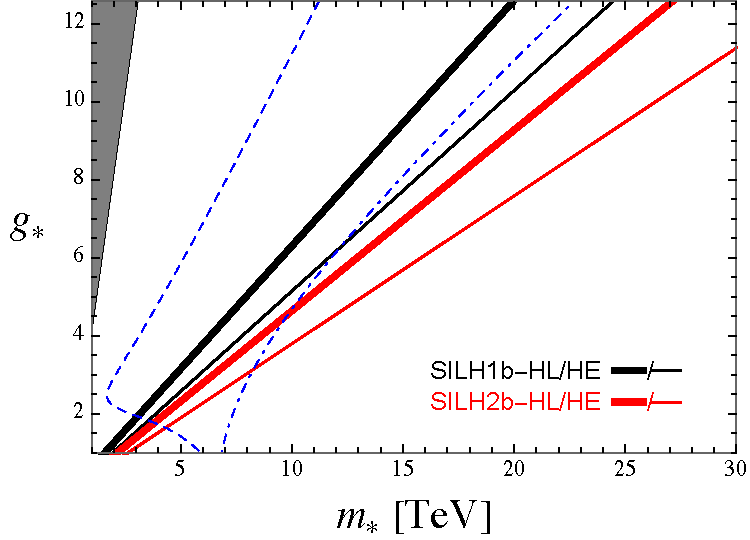
\includegraphics[scale=0.7]{\main/section2/plots/SILH1.pdf}
\caption{The constraints of table~\ref{bencharkVecchi} are interpreted as lower bounds on the new physics scale $m_*$ for a given coupling $g_*$ of the strong dynamics, see \eqref{xi}. The blue lines define lower bounds on $m_*$ from current EW precision tests for two different assumptions on the UV dynamics (see text). The grey region identifies the unphysical regime $\xi>1$. 
}\label{SILH}
\end{center}
\end{figure}
%%%%%%%%%%%%%%%%%%
%%%%%%%%%%%%%%%%%%



In Fig~\ref{SILH} we also include (blue dashed and dot-dashed lines) the current $95\%$ CL limits derived from precision EW data~\cite{Baak:2014ora} and encoded in the oblique parameters (with $U=0$)
\begin{eqnarray}
&&{\widehat S}=(1-c_V^2)\frac{g^2}{96\pi^2}\ln\frac{m_*}{m_Z}+{\widehat S}_{\rm UV}%\to-(c_V-1)\frac{1}{3\pi}\ln\frac{m_*}{m_Z}
\\\nonumber
&&{\widehat T}=-(1-c_V^2)\frac{3g'^2}{32\pi^2}\ln\frac{m_*}{m_Z}+{\widehat T}_{\rm UV}.%\to+(c_V-1)\frac{3}{4\pi c_w^2}\ln\frac{m_*}{m_Z}
\end{eqnarray}
Note that these include 1-loop effects within \eqref{eq:kappa.EFT.2} as well as contributions from heavy particles of mass $\sim m_*$ that we parametrized via $\widehat S_{\rm UV}={m_W^2}/{m_*^2}$ and $\widehat T_{\rm UV}$. The blue dot-dashed line refers to scenarios in which additional violations of custodial symmetry are negligible, $\widehat T_{\rm UV}=0$, whereas the blue dashed line to the more natural expectation $\widehat T_{\rm UV}=\xi 3y_t^2/(16\pi^2)$. Precision EW data already exclude a sizable portion of parameter space. However, as our plot clearly illustrates, these {\emph{indirect}} bounds significantly depend on unknown physics at the cutoff scale $m_*$. Hence, a {\emph{direct}} probe of the Higgs couplings provides a more robust and model-independent assessment of a given CH scenario.








\subsubsection*{The SILD}

The dominant interactions of the dilaton (still denoted by $h$) to the SM are derived from an EFT with non-linearly realized EW symmetry, where the Nambu-Goldstone bosons eaten by the $W^\pm,Z^0$ are encapsulated into the unitary matrix $\Sigma$, which transforms as $\Sigma\to U_w\Sigma U_Y^\dagger$ under $SU(2)_w\times U(1)_Y$. The powers of the singlet $h$ are fully determined by the approximate conformal symmetry. Neglecting possible (small) sources of custodial symmetry breaking, one identifies the dominant interactions:~\cite{Goldberger:2008zz}
\begin{eqnarray}\label{SILD1}
{\cal L}_{\rm SILD}&=&\frac{v^2}{4}{\rm tr}[D_\mu\Sigma^\dagger D^\mu\Sigma]\left(1+\frac{h}{f_D}\right)^2-\sum_{\psi=u,d,l}m_\psi\bar\psi_L\Sigma\psi_R\left(1+\frac{h}{f_D}\right)^{1+\gamma_\psi}\\\nonumber
&+&\frac{g_s^2}{16\pi^2}\delta_sG^a_{\mu\nu}G^{a\mu\nu}\frac{h}{f_D}+\frac{e^2}{16\pi^2}\delta_e\gamma_{\mu\nu}\gamma^{\mu\nu}\frac{h}{f_D}\\\nonumber
&+&\cdots,
\end{eqnarray}
where the dots refer to operators that impact negligibly our analysis. In the unitary gauge, the first operator in \eqref{SILD1} describes the main coupling between $h$ and the EW vector bosons. The couplings to fermions depend on how the latter interact with the underlying (approximately) conformal dynamics and are therefore model-dependent. A family-universal interaction in \eqref{SILD1} is expected in any UV theory that does not suffer from sizable flavor-changing effects, which would otherwise be in tension with precision flavor observables. Interactions with the unbroken gauge bosons in the second line of \eqref{SILD1} also depend on the details of the UV dynamics. We do not make any restrictive assumption here (besides an approximate CP symmetry) and instead allow the parameters $\delta_{g,\gamma}$ to acquire any real value. We however included a loop factor to emphasize we expect them to arise at the loop level. Similarly to what we have already stressed above \eqref{SILHvecchi}, novel corrections to $\gamma Z$ are not important to our analysis and can be ignored in a first assessment: the Lagrangian \eqref{SILD1} is enough to capture the dominant on-shell signatures of the SILD scenario as well. From \eqref{SILD} one obtains a Lagrangian like \eqref{eq:kappa.EFT.2} with 
\begin{eqnarray}\label{4parSILD}
c_V=\frac{v}{f_D},~~~~~c_y=(1+\gamma_y)\frac{v}{f_D},~~~~~c_g=2\delta_g\frac{v}{f_D},~~~~~c_\gamma=\delta_\gamma\frac{v}{f_D}.
\end{eqnarray}
Under the simplifying assumption of flavor universality ($\gamma_{u,d,e}=\gamma_y$) our EFT contains only 4 independent real parameters. %Consistently with our assumption that $f_D$ denotes the scale of spontaneous (approximate) conformal symmetry of the strong Higgs sector, we will restrict our attention to the regime $f_D\geq v$. 


We are now able to draw a few conclusions. First, as anticipated, experimental constraints on $c_V$ force $f_D\simeq v$, see Fig. \ref{SILD}. Therefore the SILD, as any other framework based on the non-linear chiral Lagrangian (i.e. where $h$ is not part of a Higgs doublet), implies the characteristic mass of the new physics lies at the relatively low scale $g_*v\lesssim4\pi v\sim3$ TeV. On the one hand this is an exciting possibility because it suggests its UV completion is more likely to be accessible at the LHC. On the other hand, a strong dynamics at such low scales contributing to EW symmetry breaking is in serious tension with EW precision data (e.g. $\widehat S_{\rm UV}\sim m_W^2/m_*^2\sim g^2/(16\pi^2)$ is typically too large as in technicolor). One can only hope the UV theory somehow cures this problem, though no concrete mechanism to achieve this is known.


%%%%%%%%%%%%%%%%%%
%%%%%%%%%%%%%%%%%%
\begin{figure}[t]
\begin{center}
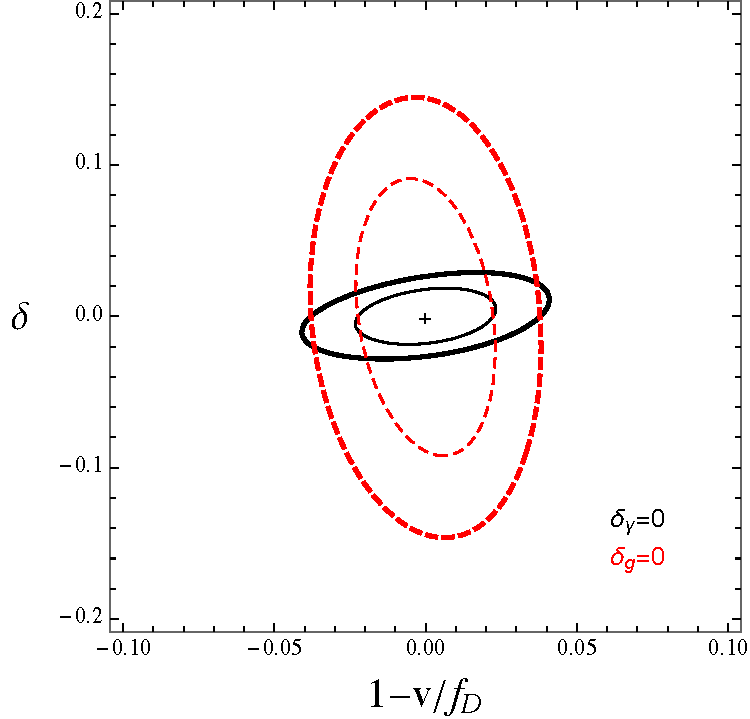
\includegraphics[scale=0.6]{\main/section2/plots/SILD.pdf}
\caption{Expected sensitivity at the $95\%, 99\%$ CL of the LHC (blue dotted), HL-LHC (black dashed) and HE-LHC (red solid) on SILD scenarios. For definiteness we set $\delta_\gamma=\gamma_y=0$.
}\label{SILD}
\end{center}
\end{figure}
%%%%%%%%%%%%%%%%%%
%%%%%%%%%%%%%%%%%%


Secondly, explicit realizations of the SILD are characterized by sizable couplings to the massless gauge bosons, $|\delta_{g,\gamma}|={\cal O}(1)$, and this appears to be in conflict with data. For example, the prototypical SILD scenario --- in which the entire SM is part of the conformal sector --- has $\delta_{g}=+46/3, \delta_\gamma=-34/9$~\cite{Goldberger:2008zz} and is already excluded with large confidence. Scenarios with partially composite SM, $|\delta_{g,\gamma}|\sim0.1$, will be subject to the significant constraints from the HL and HE upgrades, see Fig. \ref{SILD}. Unfortunately, even in this case there is no known symmetry argument that may be invoked to ensure $|\delta_{g,\gamma}|\ll1$. The only way to accommodate such a constraint within explicit strongly-coupled models seems to be via fine tuning.





Overall, the SILD scenario --- and all scenarios based on a non-linear realization of the EW symmetry --- suffers from a major drawback compared to the SILH: the SM is recovered by {\emph{tuning}} several (often uncorrelated) parameters. This is because the former do not possess a simple decoupling mechanism (analogous to the $\xi\to0$ limit in the SILH) that switches off the new physics corrections to precision data as well as $c_{V,y,g,\gamma}$. The {\emph{simultaneous}} non-observation of new physics at the TeV scale and of deviations from the SM in the future LHC upgrades would then unambiguously prove that the Higgs boson must be the missing component of the doublet responsible for EW symmetry breaking. In such a situation the only compelling realization of the CH paradigm is represented by the SILH class.




